\section{Durchführung}
\label{sec:Durchführung}

Für die Durchführung stehen mehrere Acrylzylinder in verschiedenen Größen zur
Verfügung, außerdem zwei Ultraschallsonden und ein Computer mit
entsprechendem Messprogramm. Die Acrylzylinder werden alle mit einer
Schieblehre ausgemessen.

\subsection{Geräteeinstellung}

Zunächst wird an ein beliebiger Acrylzylinder die Sonde angelegt, dabei
wird Wasser als Kontaktmittel verwendet. Nun werden die erhaltenen Impulse auf dem
Computerbildschirm sichtbar gemacht und die dazugehörige Spannung $V$ sowie
die Laufzeiten $t$ zweier reflektierter Impulse. Außerdem wird der Zylinder
mit einer Schieblehre vermessen.\\
Nachdem das Echoskop so eingestellt wurde, dass der zweite reflektiert Impuls
zwischen 1 und 1,2\;V liegt wird die Graphik gespeichert.


\subsection{Impuls-Echo-Verfahren: Bestimmung der Dämpfung}
Nun wird erneut die Sonde an den Acrylzylinder angelegt, Wasser dient als Kontaktmittel.
Aus dem auf dem Bildschirm angezeigten Diagramm wird die Amplitude
des ausgesendeten und reflektierten Impulses gemessen.
Für sechs weitere Zylinder wird diese Messung wiederholt.

\subsection{Impuls-Echo-Verfahren: Schallgeschwindigkeitsbestimmung}
Nachdem die Sonde wieder mit Wasser an den Acrylzylinder angekoppelt wurde, wird
aus dem Diagramm die Laufzeit des Echos abgelesen. Für sieben weitere
Zylinder wird äquivalent vorgegangen. (Die Zylinder werden dafür aufeinander gestapelt.)

\subsection{Durchschallungsverfahren: Schallgeschwindigkeitsbestimmung}
Für diese Messung wird der Zylinder waagerecht in die Halterung eingespannt, die
beiden Sonden werden ebenfalls in die Halterungen eingespannt und von beiden
Seiten an den Boden/Deckel des Zylinders herangeführt. Es werden für alle Zylinder
die Laufzeiten $t$, die der Schall zum Durchlaufe des Zylinders benötigt, gemessen.
Sie werden aus dem Diagramm am Bildschirm abgelesen.

\subsection{Impuls-Echo-Verfahren: Analyse und Cepstrum}
Ein 40\;mm hoher Zylinder wird auf zwei Acrylscheiben gestellt. An den
Zylinder wird die Sonde angekoppelt und die Verstärkung wird so eingestellt, dass
3 Mehrfachreflexionen zu sehen sind. Das so erhaltene Diagramm wird
gespeichert. Durch Wählen der entsprechenden Funktionen des
Analyseprogramms wird das Spektrum sowie das Cepstrum der Sonde dargestellt
und gespeichert.

\subsection{Impuls-Echo-Verfahren: Untersuchung des Augenmodells}
Um die Abstände im Auge anhand eines Modells zu bestimmen, wird Gel auf die
Ultraschallsonde gegeben und nun vorsichtig auf die Hornhaut des
Auges gesetzt. Im Abbildung \ref{fig:auge} ist Skizze des menschlichen
Auges zu sehen. Die Sonde wird leicht bewegt, bis ein Echo, dass durch
die Rückwand der Retina erzeugt wird zu sehen ist.

\begin{figure}[H]
  \centering
  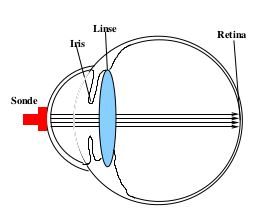
\includegraphics[height=6cm]{auge.png}
  \caption{Skizze des menschlichen Auges.}
  \label{fig:auge}
  \cite{skript}
\end{figure}
